
\documentclass[10pt]{llncs}


\usepackage{cite}
\usepackage{graphics} % for pdf, bitmapped graphics files
\usepackage{epsfig} % for postscript graphics files
\usepackage{times} % assumes new font selection scheme installed
\usepackage{amsmath} % assumes amsmath package installed
\usepackage{amssymb}  % assumes amsmath package installed
\usepackage[tight,footnotesize]{subfigure}
\usepackage{graphicx}
\usepackage{url}
\graphicspath{{.}{images/}} % declare the path(s) where your graphic files are
\begin{document}
%
% paper title
% can use linebreaks \\ within to get better formatting as desired
%\title{Efficient Representation of Chain Code with Digits of Unequal Cost}
\title{Failure Behaviour Analysis of Automated Pond Oxygen Management System}

\author{Sohag Kabir\inst{1}\and Youcef Gheraibia\inst{2}\and Tanzima Azad\inst{3}}
\institute{Department of Computer Science, University of Hull, Hull, UK\and Department of Computer Science and Mathematics,  Mohamed-Cherif Messaadia University, Souk Ahras, Algeria\and Department of Computer Science and Engineering, Bangladesh University of Enegineerinag \& Technology, Dhaka, Bangladesh\\
\email{s.kabir@hull.ac.uk, youcef.gheraibia@univ-soukahras.dz, azad.tanzima@dbbl.com.bd}
}
\maketitle


\begin{abstract}
%\boldmath
Dependability of safety-critical systems is a prime concern of the modern society due to the growing dependence on those systems. Safety of systems is a fundamental requirement for system reliability. Fault tree analysis (FTA) is well-established, powerful, and widely used tool for evaluating system safety. Fault trees provide a graphical and logical framework for analysing the dependability of systems. They have been successfully employed in studying failure behaviour of a variety of real-world systems. In aquaculture, the volume of oxygen contained in water is considered as a critical parameter for the health and well-being of fishes. If oxygen levels drop below 4 mg/L then fishes may stop feeding, stressed and begin to die. Automated Pond Oxygen Management System (APOMS) is a critical component in aquaculture to maintain the proper oxygen level in water. In summer months, when oxygen level starts dropping due to increased temperature, then the APOMS can balance the oxygen level in water by generating oxygen artificially. Therefore, the failure of this system may result in a disastrous outcome. In this paper, we have used fault tree analysis to evaluate the reliability of a generic automated fault tolerant pond oxygen management system.
\end{abstract}

\section{Introduction}
\label{sec:1}
The increasing complexity of systems has considerable significance for safety analysis as a part of dependability assessment. Dependability assessment of safety-critical
systems should begin early in the design phase so that potential problems can be identified and rectified as soon as possible to avoid expensive changes later in the system life-cycle. If problems are not rectified, system failures can result in unacceptable costs in terms of loss of life, environmental damage, and loss of resources\cite{Bernardi2007}. Most of today's systems have multiple modes of operation and many offer some level of robustness built into the design. Many systems have achieved the capability to operate in a degraded mode without failing completely by adopting some sort of fault-tolerant strategy like using redundant components or using parallel architectures. However, such complexity also poses new challenges for systems analysts, who need to understand how such systems behave and estimate how reliable and safe they really are. System analysis can help reliability engineers understand how systems work and how they can fail, thus allowing them to determine necessary actions to prevent that failure\cite{Martin2009}.

Fault tree analysis (FTA) is well-established and very popular technique for evaluating the safety  and  reliability of complex safety critical systems\cite{Leveson1995}. Fault  trees  utilise  graphical representations  based  on  Boolean  logic  to  show  logical connections  between  different  faults  and  their  causes. They are  a deductive analysis method, which means analysis starts  with  a  system  failure  known  as  the  `top  event'  and works  backwards  to  determine  its  root  causes\cite{Vesely2002}.  From  a  fault tree, it is possible to understand how combinations of failures of  different  components  or  certain  environmental 
circumstances can lead to system failure. Qualitative analysis of  fault tree is performed using Boolean logic by reducing it to minimal cut sets (MCSs) which are the smallest combinations of failure of system components that are necessary and sufficient to cause the system failure. Quantitative  analysis  of  a fault  tree,  which  follows  qualitative  analysis,  can  help  to estimate  the  probability  of  the  top  event  occurring  from  the given failure rates of basic failure modes of the system\cite{Vesely1981}.

Commercial aquaculture is growing worldwide and  according to the Food and Agriculture Organization (FAO), in 2012 aquaculture supplied the world with about 154 million tonnes of fish, of which 131 tonnes was consumed as human food\cite{Fao2012}. Ponds are the most common production systems used globally for fish production. Managing water quality in the pond is one of the most challenging tasks due to their exposure to factors of climate and topography\cite{culberson1996}. Growth rates and survival of the organisms within the pond environment is largely depending on the amount of available oxygen, dissolved oxygen levels and temperatures of pond water\cite{boyd1992, boyd1978}. Specially, in the summer time, when the water temperature goes up, then dissolved oxygen level in the pond water goes down.  Due to this reduced oxygen level fish may stop feeding and begin to die. Fish farmers could prevent oxygen depletion through monitoring and controlling oxygen level by using dissolved oxygen management systems. Therefore the success of oxygen monitoring and controlling process is primarily depends on the successful operation of the oxygen management systems. The failure of this system could lead to a catastrophic outcome. Considering the importance of such a system in fish farming, in this paper, we have performed the reliability analysis of an automated pond oxygen management system.    

The paper is organised as follows: Section \ref{sec:2} presents the fundamentals of fault tree analysis. A description of the automated oxygen management system is provided in Section \ref{sec:3}. In Section \ref{sec:4}, the result of the analysis is presented. Finally, concluding remarks are presented in Section \ref{sec:5}.

\section{Fault Tree Analysis}
\label{sec:2}
FTA is the most widely used deductive top down analysis method which allows analysts to perform both qualitative and quantitative analysis\cite{Alain1991, Vesely2002}. Fault trees (FTs) utilise graphical model to show how low-level component failure combines together to cause a top level system failure. FTA starts with an undesired event, such as system failure, known as the `top event', and then works backwards to deduce the causes of the top event in terms of logical combination of basic events\cite{Martin2009}. Symbols used in classical FTs to represent different events are shown in Fig.\ref{fig1}. 

A basic event is an initiating or basic fault that does not require any further development or expansion. It is represented as a leaf node in the fault tree. An intermediate event is a fault that is caused by the logical combinations of other events occurring further down the tree. As intermediate events are caused by other events therefore they are almost always a type of logical gate. An undeveloped event is an event whose contributions are not considered in the analysis, either because it is considered as unnecessary, or because insufficient information is available. Normal event does not represent any fault and it is part of the nominal behaviour of the system.  A conditioning event does not necessarily represent a fault, it serves as a special condition or constraint for certain types of gates. Symbols used in classical FTs to represent different logic gates are shown in Fig.\ref{fig2}.  The outcome of OR gate is true if any of the input events are true, whereas an AND gate is true if all of its input events are true. The XOR gate is true if one and only one of its input events is true. The outcome of PAND gate is true if all of its events   are true and they occur in a specific sequence. The INHIBIT gate produce an output when the input event is true in the presence of a conditioning event. Example of a fault tree is shown in Fig.\ref{fig3}\cite{John1998}.


\begin{figure}[thpb]
      \centering
      \framebox{
			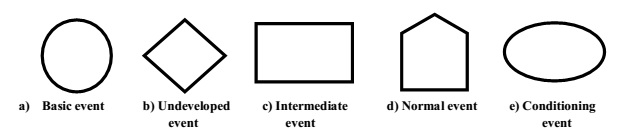
\includegraphics[scale=0.70]{events1}%[scale=0.6]
 	  }
      \caption{Fault Tree Event Symbols}
      \label{fig1}
   \end{figure}


\begin{figure}[thpb]
      \centering
      \framebox{
			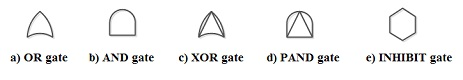
\includegraphics{gates}%[scale=0.6]
 	  }
      \caption{Fault Tree Logic Gate Symbols}
      \label{fig2}
   \end{figure}

\begin{figure}[thpb]
      \centering
      
			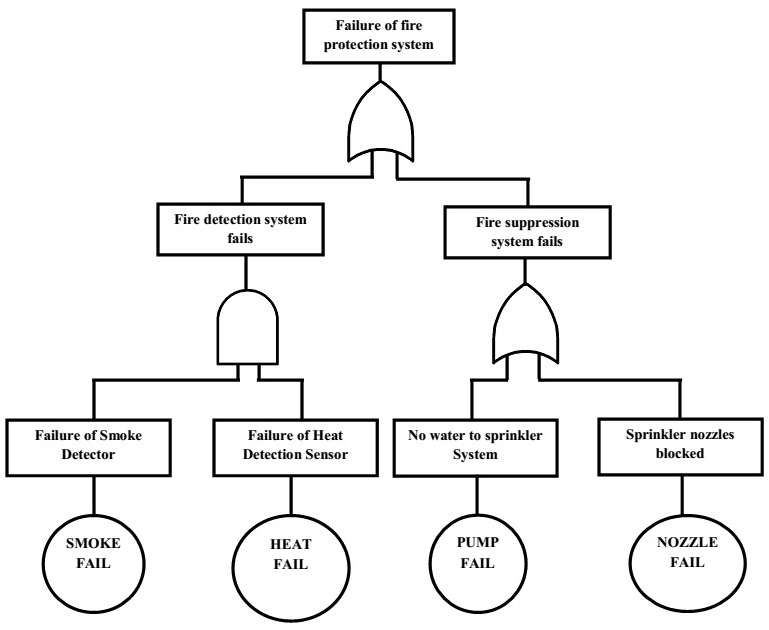
\includegraphics[scale=0.4]{example_FT1}%[scale=0.6]
 	 
      \caption{Example of a Fault Tree}
      \label{fig3}
   \end{figure}	
	
The roles of FTA in decision making are\cite{Vesely2002}: 

\begin{itemize}
\item To understand the logic leading to the top event. 
%\item Determination of effective number of iterations for coding with unequal letter cost. 
\item To prioritise the contributors leading to the top event.
\item As a proactive tool to prevent the top event.
\item To monitor the performance of the system.
\item To minimise and optimise resources.
\item To assist the designing of the system.
\item As a diagnostic tool to identify and correct causes of the top event  
\end{itemize}

Steps required for successful FTA and the interrelationship between the steps are shown in Fig.\ref{fig4}\cite{Vesely2002}. The first step is to define the objective of the FTA, i.e., defining the objectives in terms of a failure of the system to be analysed. The top event of the FT is defined in step 2 just after defining the objective of FTA. After that the scope of the FTA is defined by indicating which of the component failures and contributions will be considered and which will not be considered. The level of detail to which the failure causes for the top event will be developed is defined is step 4 as the resolution of FTA. In step 5, ground rules for the FTA are defined by declaring the procedure and nomenclature by which events and gates are named. The ground rules are very important in creating an understandable FT. The actual construction of FT is performed in step 6 and the evaluation is done in Step 7. Both qualitative and quantitative evaluations could be performed. the qualitative evaluation provides information about the minimal cut sets which are necessary and sufficient to cause the top event. The quantitative evaluation usually provides the probability of the top event and importance measure of events based on their contribution to the top event. Quantitative analysis is out of scope of this paper. Finally, at the last step the results are interpreted and presented.   
%\begin{figure}[thpb]
      %\centering
      %\framebox{
			%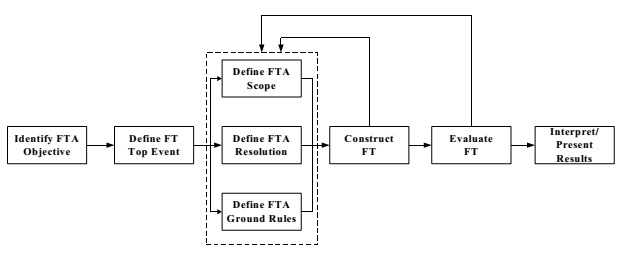
\includegraphics{block_diagram}%[scale=0.45]
 	  %}
      %\caption{Example of a Fault Tree}
      %\label{fig4}
   %\end{figure}	
	
	\begin{figure}[thpb]
      \centering
     
			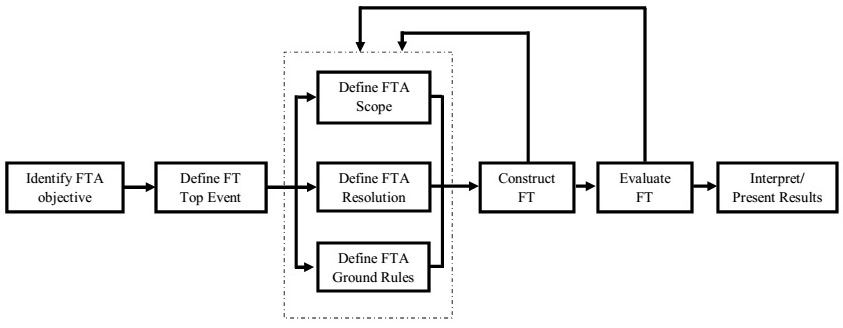
\includegraphics[scale=0.5]{block_diagram1}%[scale=0.45]
 	  
      \caption{Fault Tree Analysis Steps}
      \label{fig4}
   \end{figure}	
%%\begin{figure}[thpb]	
%\centerline{\subfigure[Basic event]{
\includegraphics{basic_event}
%\label{fig1_a}}
%\hfil
%\subfigure[Intermediate event]{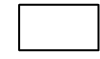
\includegraphics{intermediate_event1}
%\label{fig1_b}}}
%\caption{Classical Fault Tree Event Symbols}
%\label{fig1}
%\end{figure}
      %
%\begin{figure}[thpb]	
%\centerline{\subfigure[OR gate]{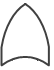
\includegraphics{or}
%\label{fig2_a}}
%\hfil
%\subfigure[AND gate]{
\includegraphics{and}
%\label{fig2_b}}}
%\caption{Classical Fault Tree Logic Gate Symbols}
%\label{fig2}
%\end{figure}

			
%\begin{table}[thpb]
%\renewcommand{\arraystretch}{1.3}
%\caption{Fault Tree Symbols}
%\label{table1}
%\centering
%\begin{tabular}{|c|c|c|}
%\hline
 %\textbf{Symbol} & \textbf{Name} & \text{Description}\\
%\hline
%
    %% \raisebox{-\totalheight}
	%\raisebox{-0.7\totalheight}	{
\includegraphics{basic_event}} & Basic Event & \begin{tabular}{@{}c@{}}A basic initiating fault requiring no \\ further development\end{tabular}\\
	%\hline
	%\raisebox{-0.7\totalheight}	{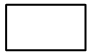
\includegraphics{intermediate_event}} & Intermediate Event &\begin{tabular}{@{}c@{}}An event arising from the combination \\ of basic events\end{tabular}\\ 
	%\hline
	%\raisebox{-0.7\totalheight}	{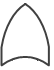
\includegraphics[scale=0.6]{or}} & AND&\begin{tabular}{@{}c@{}}Output fault occurs if all of the input  \\ faults occur\end{tabular} \\ 
	%\hline
	%\raisebox{-0.7\totalheight}	{
\includegraphics[scale=0.6]{and}} & OR&\begin{tabular}{@{}c@{}}Output fault occurs if a least one of the  \\ input faults occur\end{tabular} \\  
%\hline
%\end{tabular}
%\end{table}

FTA has been widely used in different areas to perform both qualitative and quantitative dependability analysis of the systems. Systems that have been analysed using FTA include but not limited to propulsion systems on spacecraft, braking systems in cars, Nuclear Power Plants, and so on. Different tools like HiP-HOPS\cite{Papadopoulos2012}, Reliability Workbench\cite{Isograph2014}  are available to perform fault tree analysis. FTA has been used to analyse the reliability of the power system in  \cite{volkanovski2009,cepin2011assessment}, power supply system to railways in  \cite{Chen2007}, and cogeneration power plant in textile mill in \cite{Ramesh2011}.  Recently, fault tree analysis has been applied on Clinical workflows to ensure the safety of these high-risk workflows \cite{lamis2014} and it is also used to prevent wrong-side surgery to patients \cite{abecassis2015}. Authors in \cite{shu2006using} uses FTA to analyse the potential failure scenarios in the assembly process of the printed circuit board industries. In the biological domain, FTA is used to analyse the failure of biomedical operation such as analysis for biological invasions  \cite{hayes2002identifying}. 
 

\section{Case Study: Automatic Pond Oxygen Management System}
\label{sec:3}
An automated fault-tolerant pond oxygen management system is shown in Fig.\ref{fig5}. The role of this system is to automatically generate oxygen whenever the oxygen level of pond water starts falling. Broadly, this system has a power generation unit and two subsystems (subsystem 1 and 2). The power generation unit consists of an electricity generator and a main electricity supply line. In normal condition, the system is powered by the electricity from the main line. If the main line fails (disconnected or load-shedding) then the generator is enabled to provide electricity to the system. Subsystem 1 and 2 are identical because subsystem 2 is introduced to make the system fault-tolerant. 
%Subsystem 2 is a redundant block and works as a spare component for the system. If subsystem 1 fails then subsystem 2  takes over its tasks. 
Subsystem 1 has an oxygen level sensing block ${OSB}_1$. ${OSB}_1$ block has 2 oxygen dissolver sensor ${OS}_i \left(i=1,2\right)$. Each oxygen dissolver sensor ${OS}_i$ consists of a battery unit and a sensor. For simplicity, the battery unit and the sensor of the oxygen dissolver sensors are not shown in the figure. The oxygen level sensing block ${OSB}_1$ senses the oxygen level of the pond by using oxygen dissolver sensor ${OS}_1$ and sends the reading to the decision making block ${DM}_1 $. If  ${OS}_1$ fails then ${OS}_2$  performs the task of sensing. Therefore, ${OSB}_1$ can still operate if one of its sensors fails. Characteristics and functionality of ${OSB}_2$ are similar to that of ${OSB}_1$. Decision making block can decide whether to turn on an oxygen generator after getting the oxygen level reading from the ${OSB}_1$. If required ${DM}_1$ can turn on an oxygen generator from the oxygen generator block ${OGB}_1$. Failure of ${DM}_1$ would cause the subsystem 1 to fail because there is no spare component to take over its tasks. ${OGB}_1$ block has a dedicated (private) oxygen generator $\left({OG}_1\right)$ and a shared oxygen generator $\left({OG}_3\right)$. In normal condition, ${OG}_1$ is used to generate oxygen. If  ${OG}_1$fails then  ${OGB}_1$ can use ${OG}_3$ to generate oxygen. Similarly, if ${OG}_2$ of ${OGB}_2$ fails then ${OGB}_2$ can use ${OG}_3$ to generate oxygen.   

\begin{figure}[thpb]
      \centering
   
			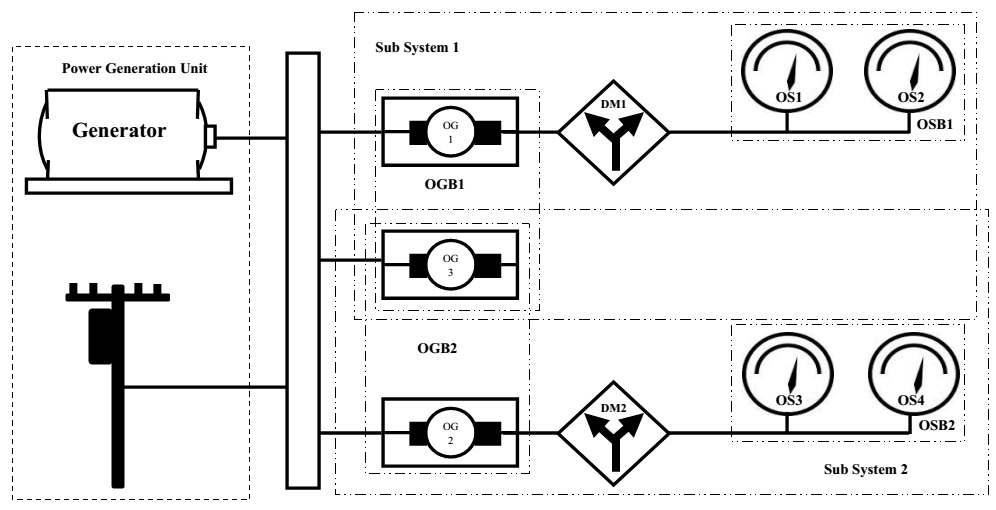
\includegraphics[scale=0.45]{pond_system1}
 	 
      \caption{Automated Fault Tolerant Pond Oxygen Management System}
      \label{fig5}
   \end{figure}	
	

%\begin{figure*}[thpb]
%\centering
%% Use the relevant command for your figure-insertion program
%% to insert the figure file.
%% For example, with the graphicx style use
%\framebox{
			%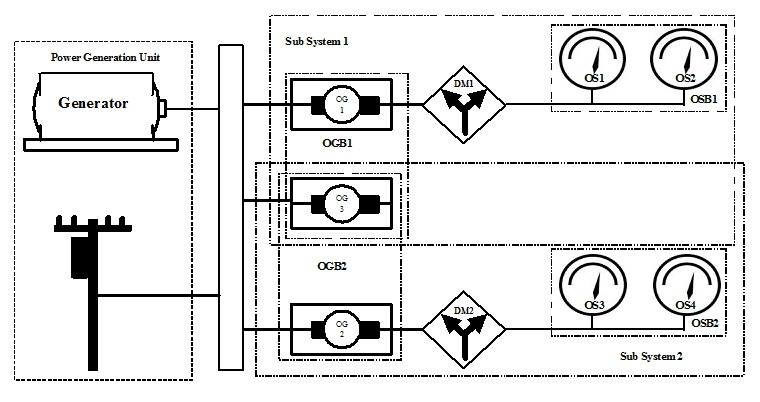
\includegraphics[scale=0.60]{pond_system}
 	  %}
%\caption{Automated Fault Tolerant Pond Oxygen Management System }
%\label{fig5}       % Give a unique label
%\end{figure*}

	
\section{ Fault Tree Generation and Evaluation}
\label{sec:4}
Before constructing the FT for the system in Fig.\ref{fig5}, we have defined the objective of the FTA for this system. The objective of the analysis is to find the possible causes that could prohibit the system from generating oxygen when required. To do this we have identified the top event as system failure, i.e. inability of the system to generate oxygen. In this paper, events are assumed to be statistically independent, and to be non-repairable---all common assumptions in FTA. At the same time, we also considered that a component could be either in failed or fully functional state, no other state is possible. The ID and names of the basic events, intermediate events, and top event are shown in Table \ref{table1} and Table \ref{table2} respectively. The fault tree of the system in Fig.\ref{fig5} is shown in Fig.\ref{fig6}.   	 

\begin{table}[thpb]
\renewcommand{\arraystretch}{1.5}
\caption{ID and Name of Basic events}
\label{table1}
\centering
\begin{tabular}{c   c}
\hline
\bfseries Event ID & \bfseries Event Name\\
\hline
MS & Failure of main electricity line\\
%\hline
EG & Failure of electricity Generator\\
%\hline
DM1 & Failure of Decision Maker in subsystem 1\\
%\hline
DM2 & Failure of Decision Maker in subsystem 2\\
%\hline
OG1 & Failure of Oxygen Generator 1 in ${OGB}_1$\\
%\hline
OG2 & Failure of Oxygen Generator 2 in ${OGB}_2$\\
%\hline
OG3 & Failure of Oxygen Generator 3 (shared)\\
%\hline
S1 & Failure of sensor in $OS_1$\\
%\hline
S2 & Failure of sensor in $OS_2$\\
%\hline
S3 & Failure of sensor in $OS_3$\\
%\hline
S4 & Failure of sensor in $OS_4$\\
%\hline
B1 & Failure of battery unit in $OS_1$\\
%\hline
B2 & Failure of battery unit in $OS_2$\\
%\hline
B3 & Failure of battery unit in $OS_3$\\
%\hline
B4 & Failure of battery unit in $OS_4$\\
\hline
\end{tabular}
\end{table}

\begin{table}[thpb]
\renewcommand{\arraystretch}{1.3}
\caption{ID and Name of Intermediate and top events}
\label{table2}
\centering
\begin{tabular}{c c}
\hline
\bfseries Event ID & \bfseries Event Name\\
\hline
TE & System Failure---no oxygen supply\\
%\hline
SSF & Failure of Subsystem 1 and 2\\
%\hline
PS & Failure of Power Supply Block\\
%\hline
SS1 & Failure of Subsystem 1\\
%\hline
SS2 & Failure of Subsystem 2\\
%\hline
OSB1 & Failure of ${OSB}_1$ block\\
%\hline
OSB2 & Failure of ${OSB}_2$ block\\
%\hline
OGB1 & Failure of ${OGB}_1$ block\\
%\hline
OGB2& Failure of ${OGB}_2$ block\\
%\hline
OS1 & Failure of oxygen dissolver $OS_1$ \\
%\hline
OS2 & Failure of oxygen dissolver $OS_2$\\
%\hline
OS3 & Failure of oxygen dissolver $OS_3$\\
%\hline
OS4 & Failure of oxygen dissolver $OS_4$\\
\hline
\end{tabular}
\end{table}

\begin{figure*}[thpb]
\centering
% Use the relevant command for your figure-insertion program
% to insert the figure file.
% For example, with the graphicx style use
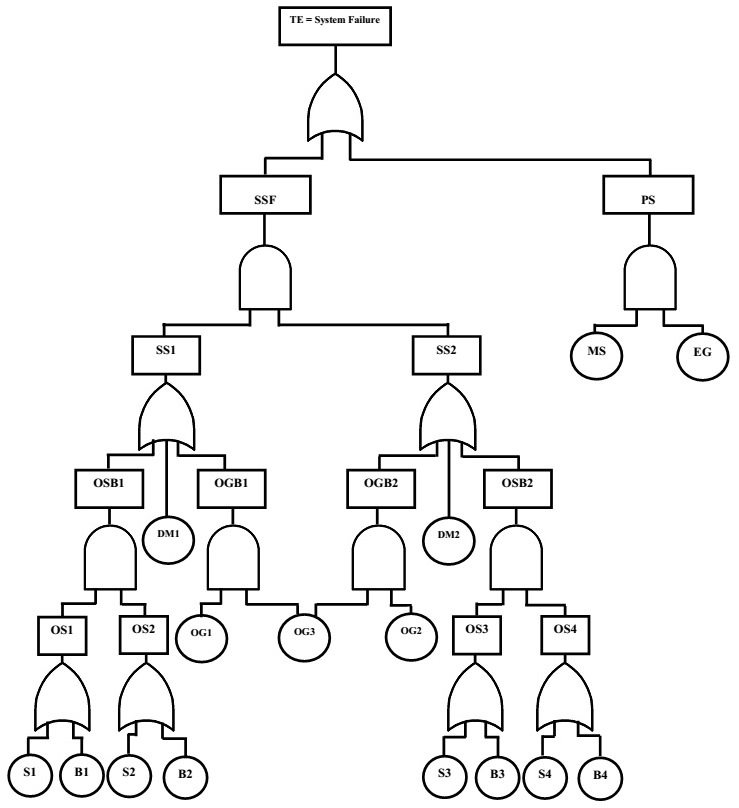
\includegraphics[scale=.65]{FTA_main}
\caption{Fault Tree of the System in Fig.\ref{fig5} }
\label{fig6}       % Give a unique label
\end{figure*}

The logical expression of the top event as disjoint sum of minimal cut sets can be given by following expression:

\begin{align*}
\begin{split}
    System~ Failure=MS\cdot EG+S_1S_2S_3S_4+S_1S_2S_3B_4+S_1S_2B_3S_4+S_1S_2B_3B_4~~~~~~~~~~~~~~~~~~~~~~~~~~~~~~~~~\\+S_1S_2DM_2+S_1S_2OG_2OG_3	+S_1B_2S_3S_4+S_1B_2S_3B_4+S_1B_2B_3S_4~~~~~~~~~~~~~~~~~~~~~~~~~~~~~~~~~~~\\+S_1B_2B_3B_4+S_1B_2DM_2+S_1B_2OG_2OG_3+B_1S_2S_3S_4     +B_1S_2S_3B_4~~~~~~~~~~~~~~~~~~~~~~~~~~~~~~~~~\\+B_1S_2B_3S_4+B_1S_2B_3B_4+B_1S_2DM_2+B_1S_2OG_2OG_3+B_1B_2S_3S_4~~~~~~~~~~~~~~~~~~~~~~~~~~~~~~~~~\\+B_1B_2S_3B_4		+B_1B_2B_3S_4+B_1B_2B_3B_4+B_1B_2DM_2+B_1B_2OG_2OG_3~~~~~~~~~~~~~~~~~~~~~~~~~~~~~~\\+DM_1S_3S_4+DM_1S_3B_4+DM_1B_3S_4			+DM_1B_3B_4+DM_1DM_2~~~~~~~~~~~~~~~~~~~~~~~~~~~~~~~~~~~~~~~~\\+DM_1OG_2OG_3+OG_1OG_3S_3S_4+OG_1OG_3S_3B_4+OG_1OG_3B_3S_4~~~~~~~~~~~~~~~~~~~~~~~~~~~~~~~~~~~\\+OG_1OG_3B_3B_4+OG_1OG_3DM_2+OG_1OG_2OG_3~~~~~~~~~~~~~~~~~~~~~~~~~~~~~~~~~~~~~~~~~~~~~~~~~~~~~~~~~~~~~~~~~
\end{split}  
\end{align*}

From the above expression, we can see that there are 37 minimal cut sets which can cause the system failure. For example, the first cut set $MS\cdot EG$ corresponds to the power generation unit, if both main electricity line and electricity generator fail, then it will cause the power generation unit to fail which will eventually cause the system failure. Because without electricity the system will not be able to operate even though all other components are fully functional. Similarly, the last cut set $OG_1 \cdot OG_2 \cdot OG_3$ represents the scenario when all the oxygen generators fail. In this case, even all other components of the system work properly to detect the oxygen level of the water still the system cannot produce oxygen to balance the oxygen level because none of the oxygen generator is operational to generate oxygen.


\section{Conclusion}
\label{sec:5}
Fault tree analysis is an effective method to evaluate the safety and reliability of safety-critical systems. It has been widely used in the dependability analysis for many complex systems involved in, nuclear reactor, aerospace industry, and chemical plants. This paper demonstrates the use of the FTA for performing reliability analysis of automated pond oxygen management system. We have performed the qualitative analysis to determine the minimal cut sets that are necessary and sufficient to cause the system failure. Our analysis determines 37 different combinations of system component failures that can cause the system failure. The analysis results can be combined to improve the system design, which may lead to a system with higher quality and reliability. At present, as we do not have any quantitative information (e.g. failure rates) about the system components therefore quantitative analysis is not performed. In future, we have the plan to extend this work by collecting quantitative information about the components and performing quantitative analysis of this system.

\bibliographystyle{splncs03}
\bibliography{biblio}
\end{document}


